\chapter{Magie}
\section{Das Konzept der Magie}
\subsection{Was ist Magie?}
In diesem Universum ist Magie eine besondere Form der Energie und ist ein Nebenprodukt bei Energieumwandlungen.
Es entsteht also überall dort Magie, wo irgendeine Form der Energie in eine andere umgewandelt wird - was sowohl in der belebten als auch der unbelebten Natur ständig der Fall ist.
So führen z.B. Steinschläge oder Lawinen zu einem plötzlichen Auftreten einer gewissen Menge von Magie, während ein Vulkanausbruch hingegen eine ziemliche Masse an Magie produziert. 
Ja schon allein die Plattentektonik sorgt für das Vorkommen von Magie.
Da Magie eine Form der Energie ist, kann sie deshalb auch selbst wieder zurück in andere Energieformen umgewandelt werden.
Im Allgemeinen "`diffundiert"' die erzeugte Magie nämlich von ihrem Ort der Entstehung hinweg in die Umgebung, da es nichts gibt, was sie halten würde.
Dort wird sie nach und nach wieder umgewandelt.


\subsection{Anpassung der belebten Natur}
Es ist also kein Wunder, dass Magie hier auf \nameref{sec:planet} nichts besonderes ist, und dass sich das Leben dementsprechend auch entwickelte - denn insbesondere in und um Zellen erfolgt am laufenden Band die Umwandlung von Energie zwischen verschiedenen Formen.
Daher haben Zellen eine Möglichkeit entwickelt, Energie in Form von Magie zu halten und zu einem gewissen Grad anzusammeln.
Bei Eukaryoten (Pflanzen, Pilze, Tiere) ist dies eine Art Vakuole. 
Die maximal zu haltende Menge ist artabhängig und angeboren.
Ist diese Menge überschritten, so diffundiert alles Überschüssige wieder aus der Zelle in die Umwelt.
Die so gehaltene Menge an Magie wird auch als Mana oder Manapool bezeichnet.

Eine Verbildlichung lässt sich mit einer Zisterne darstellen: diese füllt sich mit dem Wasser vom Dach des Hauses, bis sie voll ist.
Danach läuft sie über und das Wasser verteilt sich in der Gegend.

Ursprünglich war dies ein Vorteil bezüglich des Überlebens der Zelle: im größten Notfall, wenn die Zelle keine Energiezufuhr jegweder Art erhält, dann kann sie ein energieintensives Notprogramm initialisieren, welches ihr die Magie als tatsächliche Energiereserve zu nutzen ermöglicht.
So kann die Zelle einen kurzen Zeitraum ohne Versorgung überbrücken.
Im Laufe der Evolution haben viele Lebewesen dann Mechanismen entwickelt, um die ihnen innewohnende Magie in ihrem Sinne auf einem intuitiven Level umzuwandeln bzw einzusetzen.
Bei Tieren kann man sich das wie eine Art zweites Nervensystem vorstellen, welches sich an den Adern entlang durch den ganzen Körper zieht und vom Rückenmark aus kontrolliert wird.
Dieses Geflecht wird aus besonderen Zellen gebildet, die selbst keine Magie speichern, sondern die Magie aus den restlichen Zellen des Körpers abziehen.
Diese gelangt somit in das Netzwerk, wo sie über das Rückenmark gezielt kontrolliert werden kann.

In welcher Weise sie die Magie kontrollieren können, ist genetisch festgelegt und hat sich evolutionär entwickelt.
Der Einsatz erfolgt im intuitiven Sinne wie ein Reflex oder eine Reaktion auf etwas, das passiert, oder unterstützt eine Handlung. 
So gibt es Pflanzen, die zur Abwehr von Fressfeinden kleine Elektroschocks verteilen, zum Anlocken von Bestäubern mit Licht spielen, oder Prädatoren, die mittels Infrarot-Magie ihre Beute ohne Probleme von der Umgebung unterscheiden können.

Jeder Mensch beherrscht die Magie auf diesem Level und zeigt sich erstmals im Bereich von 4-7 Jahren.
Im Verlauf der Differenzierungen der verschiedenen Menschenarten haben sich unterschiedliche Ausprägungen durchgesetzt oder sind erst entstanden.


\subsection{Aktive Verwendung}
Einige Lebewesen haben zudem die Fähigkeit entwickelt, die Magie aktiv in ihrem Interesse einzusetzen.
Bei Tieren bedeutet das, dass sich auch das Gehirn bei der Steuerung einschaltet.
Dabei wird sie auf ein Ziel ausgerichtet und dort die bestehenden Zustände geändert.
Es muss allerdings eine deutlich größere Menge an Magie eingesetzt werden, als der Vorgang bzw. die Änderung eigentlich an Energie benötigen würde.
So hat auch der Mensch schließlich festgestellt, dass er mithilfe seines Willens und Konzentration dazu in der Lage ist, diese Möglichkeiten auszubauen und zu verstärken.
Nur Personen, die sich intensiv mit ihren Fähigkeiten auseinandersetzen, viel meditieren, experimentieren und Verständnis suchen, nur diese Personen lernen, das Tauschverhältnis zu reduzieren und immer mehr zu einem halbwegs äquivalenten Austausch zu kommen.
Das führt dazu, dass sie mit dem ihnen angeborenen Manapool mehr und stärkere Dinge bewirken können.
Ihre einzigen Grenzen sind dabei durch ihre Gene, ihre Vorstellungskraft, ihre Konzentrationsfähigkeit und den magischen Widerstand anderer Lebewesen gesetzt. 
\\ \\
Es gibt ein paar Prokaryoten, die sich die Magie als tatsächliche dauerhafte Energiequelle erschlossen haben und sie ständig direkt zur Herstellung von ATP (Adenosintriphosphat = "`Energie der Zelle"') nutzen können.
Bisher ist noch kein Fall von Symbiose oder gar Endosymbiose ähnlich wie mit den Mitos (\textalpha-Proteobakterien $\rightarrow$ Mitochondrien) oder Chloros (Cyanobakterien $\rightarrow$ Chloroplasten) bekannt, aus dem höher entwickelte Lebewesen herausgekommen sind, da dies vor nicht allzu langer Zeit (in Zeiträumen der Evolution) entstand.


\subsection{Natürlicher magischer Widerstand}
Ist es im Allgemeinen nicht schwer, den eigenen Körper und die Umgebung zu beeinflussen, so ist das Verändern von Zuständen in anderen Körpern ein ganz anderes Thema.
Höher entwickelte Lebewesen, die ein Verständnis für den eigenen Körper oder sogar ein Ich-Bewusstsein erstanden haben, besitzen dadurch einen Art natürlichen magischen Widerstand gegen Änderungen, die in ihrem Körper erfolgen sollen. 
Dieser ist umso stärker, je ausgereifter das Bewusstsein ist.
Das führt dazu, dass nur wirklich mächtige und studierte Individuen es schaffen, diese Barriere zu überwinden und Magie innerhalb solcher Körper zu wirken.



\section{Magie-Kontrolle}
\paragraph{Hintergrund}
Magie kann eingesetzt werden, um bestimmte physikalische oder chemische Prozesse zu verändern - in einem gewissen Rahmen, der genetisch vererbt wurde.
Somit bedeutet die Beherrschung einer Magie-Art eigentlich, dass das Wesen dazu fähig ist, die Magie kontrolliert in diese bestimmte Art Energie umzusetzen.
Welche Arten bisher schon entstehen zeigt die kategorisierte Übersicht in Abb. \ref{fig:magiearten-uebersicht}.

\begin{figure}[htb]
	\centering
	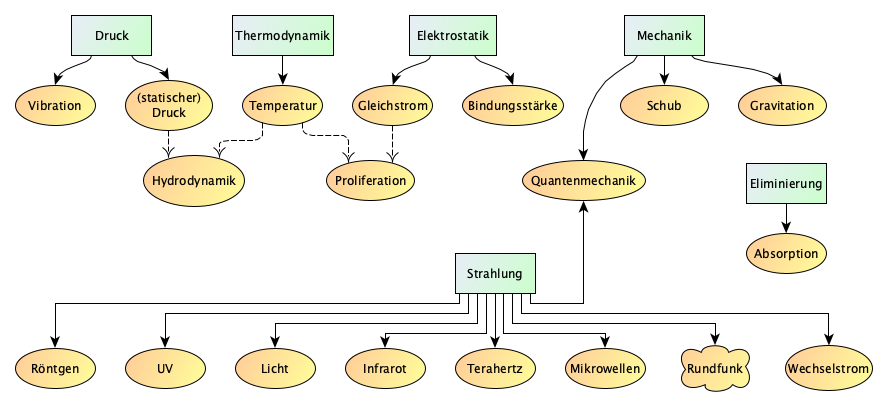
\includegraphics[width=\linewidth]{Abbildungen/Weltenbau/Magie/Magiearten-Uebersicht}
	\caption[Übersicht der Arten der Magiekontrolle]{\textbf{Alle bekannten Arten der Kontrolle über Magie in der Übersicht.} \\ 
	Verwandte Arten sind durch ihre Kategorisierung und ihre Verbindung über Pfeile gekennzeichnet.}
	\label{fig:magiearten-uebersicht}
\end{figure}


\paragraph{Stufen der Kontrolle}
Bei den folgenden verschiedenen Arten der Magie-Kontrolle, auch Magiearten genannt, ist dargestellt, wie die intuitive Nutzung dieser Eigenschaft aussieht oder wie Begabte mit ihr umgehen können.
Meisterliche Magier erreichen noch ganz andere Level. 
In der Regel sind sie schon in hohem Alter und haben sich ihr Leben lang mit der Verbesserung, dem Lernen und Ausprobieren beschäftigt, weshalb es nur wenige von ihnen gibt, die so weit kommen. 
Neben der Intensivierung und Verbesserung vorheriger Zauber gelingt ihnen auch eine Manipulation ganz anderer Art: 
Sie können die natürliche Resistenz des Körpers (siehe oben) umgehen.


\paragraph{Magie-Arten}
Die Informationen über die Verbreitung der Magiearten unter den Lebewesen und ihrer Bekanntheit in \nameref{sec:land} finden sich einerseits bei jeder Art und andererseits in Tab. \ref{tab:magie-verbreitung} zur Übersicht.

Die Anordnung der Magiearten ist alphabetisch, um einen schnellen Zugriff zu ermöglichen.

\begin{table}[htbp]
	\centering
	\caption{Verbreitung der Magiearten unter den Lebewesen allgemein und unter den Menschenarten.}
	\label{tab:magie-verbreitung}
	\begin{threeparttable}[\linewidth]
		\begin{tabularx}{\textwidth}{l|ccX}
			\toprule
			\textbf{Art} & \textbf{Hominini} & \textbf{Mensch} & \textbf{Bemerkungen} \\
		    \midrule
			Absorption & - & - & Bisher nur bei Mikroorganismen \\
			Druck & X & X & Zweithäufigste unter den Menschen, auch im Tierreich stark verbreitet \\
			Elektrizität & X & X & Mäßige Verbreitung unter den Menschen, vor allem schlecht ausgenutzt, da Elektrizität ihnen noch kein richtiger Begriff ist. Vor allem bei Pflanzen und Tieren \\
			Licht & X & X & Mäßige Verbreitung unter den Menschen \\
			Proliferation & X & X & Unter den Menschen sehr selten \\
			Strahlung & - & - &  \\
			Temperatur & X & X & Am weitesten verbreitet \\
			Verhärtung & X & - & Sylvan \\
			Vibration & X & - & Zwerge und Undar \\
			\bottomrule
		\end{tabularx}
	\end{threeparttable}
\end{table}



\subsection{Absorption oder Nullmagie}\label{sec:nullmagie}
Diese Art der Kontrolle sorgt für einen ständigen Entzug von Magie aus der Umwelt, da zumindest beim Menschen die eigenen Zellen nicht mehr fähig sind, diese zu halten und somit versuchen, auszugleichen. 

\subsubsection{Verbreitung}
Zu Beginn des Spiels beherrschen nur Mikroorganismen diese Fähigkeit. Am Ende wurde eine neue Art Mensch geschaffen, die diese Fähigkeit ebenso beherrschen. Sie ist daher anfangs vollkommen unbekannt.

\subsubsection{Bedeutung im Spiel}
Zum aktuellen Zeitpunkt nicht existent, denn sie entsteht erst bei der Gottwerdung in den Überlebenden.

\subsubsection{Intuitive Nutzung}
Die Bakterien nutzen es als Energiequelle mittels eines speziellen Zellorgans. Es lässt sich ähnlich vorstellen wie die Nutzung von Sonnenenergie mittels Chloroplasten oder chemischer Energie mittels Mitochondrien. 

Die Menschen werden durch das heftige Ziehen sämtlicher Magie relativ unbeeinflussbar durch Magie, die direkt auf sie gewirkt wird oder auf das, was sie berühren. Sie sind jedoch unfähig, selbst Magie zu wirken.

\subsubsection{Erlernbare Steigerungen}
Es wird sehr lange dauern, bis die Menschen begreifen, dass auch dies eine Möglichkeit zur Steigerung bietet.
\begin{itemize}
	\item Aktives Absorbieren von Magie aus Lebewesen, was diese daran hindert, ihre Magie einsetzen zu können.
	\item ...
\end{itemize}

\subsubsection{Meisterliche Beherrschung} 
\begin{itemize}
	\item ...
\end{itemize}




\subsection{Druck}\label{sec:druckmagie}
Diese Eigenschaft erlaubt die Kontrolle über den lokalen Druck und damit verbunden die Entstehung von Wind. Es existiert die präzisere Unterform \nameref{sec:vibrationsmagie}, sowie die weiterentwickelte Form \nameref{sec:haertungsmagie}.

\subsubsection{Verbreitung}
Ähnlich wie bei der thermischen Energie ist diese Form recht weit verbreitet. Die homininen Arten beherrschen diese Kontrolle. 

In unserem Land ist die Magieform allerdings nicht ganz so häufig wie die der Temperatur anzutreffen. Ansonsten ist sie gut bekannt.

\subsubsection{Bedeutung im Spiel}
Die \npref{sec:mc_diplomatin} hat diese Eigenschaft ab ihrem Schlüsselmoment. 

\subsubsection{Intuitive Nutzung}
Die Lebewesen können somit in einer Art Reaktion Gefahren, die zu nah an sie herankommen, von sich wegschubsen, ohne sie zu berühren, oder sich selbst aus einem gefährlichen Bereich heraus drängen. Ebenso können sie damit direkt um sich herum Wind erzeugen oder diesen negieren und sind daher von stürmischen Auswirkungen meist weniger betroffen.

Bei den Menschen findet sich eine zusätzliche Verwendung meist nur darin, lustige Effekte mit den Haaren hervor zu rufen.

\subsubsection{Erlernbare Steigerungen}
\begin{itemize}
	\item Es sind deutlich weitere und höhere Sprünge möglich.
	\item Das Erzeugen kleiner Windhosen bzw. Staubteufel.
	\item Es wird Druck auf andere Dinge angewendet, womit sie entweder auseinander gerissen oder zerquetscht werden.
	\item Gegenstände oder Lebewesen werden kontrolliert an Ort und Stelle gehalten oder durch die Gegend gedrückt.
	\item Der eigene Körper kann etwas über den Boden schweben.
	\item Einkommender Druck kann abgefangen und auf eine größere Fläche verteilt werden: zuerst nur bei größerflächigen Dingen wie Steinen oder Stöcke. Später auch gegen Waffen, die genau so was ausnutzen: Klingenwaffen. Dadurch wird weniger Schaden genommen.
	\item ...
\end{itemize}

\subsubsection{Meisterliche Beherrschung} 
\begin{itemize}
	\item Den Druck im Kopf erhöhen, bis er platzt.
	\item Den Blutdruck plötzlich extrem absenken, so dass der Gegenüber bewusstlos zusammenbricht. 
	\item Den Druck in der Umgebung so stark beeinflussen, dass sich dadurch das Wetter ändern kann. Damit lassen sich zB. Regenwolken lenken. 
	\item Eine Art Fliegen, aber mehr im Sinne eines erweiterten Schwebens.
	\item ...
\end{itemize}



\subsection{Elektrizität und Magnetismus}\label{sec:elektromagie}
Mit dieser Eigenschaft lassen sich elektrische Ströme und Ladungen beeinflussen. Ebenso kann dies für Elektromagnetismus genutzt werden.

\subsubsection{Verbreitung}
Dies ist weit unter Tieren und insbesondere Pflanzen verbreitet. Doch auch die Hominini besitzen diese Fähigkeit, allerdings ist ihnen Elektrizität oder im weiteren Sinne noch kein Begriff, weshalb das Ausbauen und Ausnutzen dieser Kontrolle recht schlecht ist.

\subsubsection{Bedeutung im Spiel}
Die \npref{sec:mc_diplomatin} hat diese Eigenschaft von Beginn an. 

\subsubsection{Intuitive Nutzung}
Die meisten Lebewesen nutzen Schockstöße zur Abwehr von Räubern und Fraßfeinden. Werden sie von Blitzen getroffen, so sterben sie nicht, sondern dienen als eine Art Ableiter. 

\subsubsection{Erlernbare Steigerungen}
\begin{itemize}
	\item Metallische (magnetische) Gegenstände von entsprechender Größe sind frei bewegbar.
	\item Metalle werden (ent-)magnetisiert.
	\item Das Erzeugen von elektrischer Energie, die an die Umwelt abgegeben werden kann.
	\item ...
\end{itemize}

\subsubsection{Meisterliche Beherrschung} 
\begin{itemize}
	\item Die Signale von Nervenzellen werden an ihnen selbst mittels Elektrizität weitergeleitet. Dieser Fluss lässt sich stören, womit zum Beispiel eine Reaktion des Gegenübers verhindert wird. Das ist allerdings recht unpräzise, da die Funktionsweise des Körpers noch nicht so weit bekannt ist. Durch das spüren der Ströme allerdings konnten einige Erkenntnisse gewonnen werden. So lässt sich zB sämtlicher elektrischer Fluss in einzelne Gliedmaßen ausschalten, wodurch diese nicht mehr bewegt werden können.
	\item Ebenso kann man damit das Gehirn von jemanden lahm legen und ihn damit effektiv töten.
	\item Das Herz wird von einem Nervenknoten, dem Sinus, kontrolliert. Bei Herzstillstand kann man es wieder zum schlagen bringen, indem man diesem Knoten einen elektrischen Impuls gibt, damit das Herz wieder zu arbeiten beginnt (siehe auch Defibrillator).
	\item ...
\end{itemize}



\subsection{Strahlung}\label{sec:strahlungsmagie}
Diese Eigenschaft ermöglicht die Kontrolle von Strahlung: Aussenden und Absorbieren. Das umfasst alle Strahlungsfrequenzen von  über ... bis hin zu y.
ermöglicht das Aussenden und Absorbieren von hochenergetischer Strahlung: energiereicher als Licht aka UV, alpha-, beta-, gamma-Strahlung. Aufteilung in verschiedene Bereiche, wie schon Licht abgetrennt ist? 

\subsubsection{Verbreitung}
...\\
Keine Verbreitung unter den Menschen.

\subsubsection{Bedeutung im Spiel}
Derzeit keine Bedeutung im Spiel.

\subsubsection{Intuitive Nutzung}
Lebewesen mit nackter Oberfläche bekommen keinen Sonnenbrand.

\subsubsection{Erlernbare Steigerungen}
\begin{itemize}
	\item Das Aussenden entsprechender Strahlung führt zu gehäuften Mutationen, was zu Tumoren führen kann.
	\item Erweitertes Sehen mittels UV-Strahlung?
	\item ...
\end{itemize}

\subsubsection{Meisterliche Beherrschung} 
\begin{itemize}
	\item Das Hervorrufen der Strahlungskrankheit.
	\item ...
\end{itemize}

\subsection{Licht und Dunkelheit} \label{sec:lichtmagie}
Diese Eigenschaft ermöglicht die Kontrolle von Licht bzw. dessen Abwesenheit.

\subsubsection{Verbreitung}
Eine recht weit verbreitete Kontrollfähigkeit unter Lebewesen. Bei den Hominini ist sie nicht so stark verbreitet wie andere.

\subsubsection{Bedeutung im Spiel}
Die \npref{sec:mc_spionin} beherrscht diese Eigenschaft. 


\subsubsection{Intuitive Nutzung}
Viele Lebewesen nutzen dies zur Attraktion von anderen Lebewesen, sei es um diese zu Nutzen oder als Beute. Einerseits Licht insbesondere bei Nacht, andererseits Illusionen um zu täuschen. \\
Man munkelt auch von einer Tierart, die sich so gut an die Umwelt anpassen, dass sie von ihrer Beute nicht entdeckt wird, bis es zu spät ist. 

Menschen nutzen dies insbesonders um sich selbst attraktiver zu machen.

\subsubsection{Erlernbare Steigerungen}
\begin{itemize}
	\item Das Erzeugen von Licht.
	\item Mit hellem Licht lassen sich Gegner blenden oder gar erblinden.
	\item Illusionen dienen zur Unterhaltung oder Ablenkung.
	\item Mittels Illusionen kann man sich dem Hintergrund anpassen, wodurch man deutlich schlechter zu sehen ist.
	\item ...
\end{itemize}

\subsubsection{Meisterliche Beherrschung} 
\begin{itemize}
	\item Wahre Meister des Fachs können das Licht so geschickt manipulieren, dass sie einem unaufmerksamen Auge gar als unsichtbar scheinen können.
	\item Die Kontrolle über die An- oder Abwesenheit von Licht in einem gewissen Bereich.
	\item ...
\end{itemize}



\subsection{Proliferation}\label{sec:proliferationsmagie}
Diese Eigenschaft ist eher chemischer Natur und erlaubt die Beeinflussung der Reaktionsgeschwindigkeit.

\subsubsection{Verbreitung}
Wenige Pflanzen- und Tierarten sind dieser Fähigkeit mächtig. Auch bei den Hominini ist es eine seltene Gabe. Aufgrund der Nachteile ist gar der Glaube verbreitet, dass diese Menschen ihr eigenes Leben geben, um andere zu heilen, weshalb nur höherrangige Leute davon profitieren dürfen.

\subsubsection{Bedeutung im Spiel}
Nur sehr wenig Individuen im Land haben diese Kontrollform in größerem Ausmaße geerbt. Diese sind hochgeschätzte Mitglieder des Ordens und erfreuen sich besten Umständen. Der Spieler erhält daher erst später Zugriff darauf, nachdem er entsprechend im System aufgestiegen ist.

\subsubsection{Intuitive Nutzung}
Diese Menschen leben kürzer als der Rest, da in ihrem gesamten Körper die Reaktionen sehr schnell ablaufen. Dadurch haben sie eine gesteigerte Reaktionszeit und heilen deutlich schneller.

\subsubsection{Erlernbare Steigerungen}
\begin{itemize}
	\item Erweitern der gesteigerten Reaktionen auf die nahe Umwelt: Pflanzen wachsen schneller.
	\item Zudem kann dies zur Heilung anderer eingesetzt werden.
	\item Allerdings können damit auch krankhafte Tumore hervorgerufen werden... 
	\item ...
\end{itemize}

\subsubsection{Meisterliche Beherrschung} 
Nur extrem wenige Menschen haben lange genug gelebt, um diese Stufe zu erreichen.
\begin{itemize}
	\item Das plötzliche starke Altern des Gegenübers.
	\item Das Verlangsamen der eigenen Alterung durch das Umkehren der obigen Prozesse. Das kehrt auch die anderen Folgen um. Es heißt, es liegt ein solcher Magier irgendwo in einer Art Winterschlaf und er wird aufwachen, wenn die Welt ihn wieder benötigt (Ref: König Barbarossa? Ggf. unter Märchen und Quests ausfeilen). %todo
	\item ...
\end{itemize}



\subsection{reine Energie}\label{sec:energiemagie}
...

\subsubsection{Verbreitung}
...\\
Keine Verbreitung unter den Hominini.

\subsubsection{Bedeutung im Spiel}
Derzeit keine Bedeutung im Spiel.

\subsubsection{Intuitive Nutzung}
...

\subsubsection{Erlernbare Steigerungen}
\begin{itemize}
	\item ...
\end{itemize}

\subsubsection{Meisterliche Beherrschung} 
\begin{itemize}
	\item ...
\end{itemize}



\subsection{Temperatur}\label{sec:temperaturmagie}
Diese Eigenschaft erlaubt die Kontrolle über die thermische Energie der Umgebung, sowohl das Erhitzen als auch das Abkühlen.

\subsubsection{Verbreitung}
Diese Manipulation der thermischen Energie ist uralt und daher weit verbreitet unter allen Arten von Lebewesen; Somit auch unter den homininen Arten. Sie ist gut bekannt.

\subsubsection{Bedeutung im Spiel}
Diese Magiekontrolle beherrscht der \npref{sec:mc_soldat}. Es ist ansonsten eine der am weitesten verbreiteten Arten unter der Bevölkerung. Allerdings wird sie unter Hominini nicht vererbt sondern ergibt sich aus der Kombination der Gene für Druck- und Luft-Kontrolle.

\subsubsection{Intuitive Nutzung}
Diese Lebewesen haben weniger Temperaturprobleme, da sie um sich herum eine kleine Blase erwärmter oder abgekühlter Luft schaffen können. Einige nutzen dieses Konzept auch zur Jagd, sowohl an Land als auch im Wasser, wo sie die Luft oder das Wasser stark erhitzen oder extrem abkühlen und damit für Verbrennungen oder Erfrierungen sorgen.

\subsubsection{Erlernbare Steigerungen}
Zuerst Beispiele für die Erhitzung:
\begin{itemize}
	\item Das Erhitzen von Gegenständen abseits vom eigenen Körper, insbesondere sehr gut Wärme-leitenden Materialien wie Metall. Dies wird zB. im Kampf ausgenutzt, um die Waffe oder die Rüstung des Gegners zu heiß zum Halten/Tragen werden zu lassen.
	\item Das Entzünden entflammbarer Objekte.
	\item Das Erschaffen kleiner Massen glühender Hitze, die weggeworfen werden kann. Beim Aufprall entzünden sich die vor Ort befindlichen Materialien. 
	\item Wandförmige Bereichen von Luft werden so stark erhitzt, dass alles, was sie berührt, schmilzt oder brennt.
	\item ...
\end{itemize}

Nun Beispiele für das Abkühlen:
\begin{itemize}
	\item Das Metall am Körper des Gegenübers erkalten lassen. Das kann zu Verbrennungen führen.
	\item Feuchte Körperteile lassen sich an gefrorenen Gegenständen, insbesondere metallischen, anfrieren.
	\item Flüssigkeiten auf dem Boden (idR Wasser) lassen sich gefrieren, womit Glatteis erzeugt wird.
	\item Feuer lassen sich durch einen gegensätzlichen Effekt löschen.
	\item ...
\end{itemize}

\subsubsection{Meisterliche Beherrschung} 
\begin{itemize}
	\item Das Blut/der Körper des Gegners kann zum Kochen gebracht werden.
	\item Körperteile des Gegners können erfroren werden.
	\item ...
\end{itemize}



\subsection{Verhärtung}\label{sec:haertungsmagie}
Mittels dieser Fähigkeit lassen sich Atombindungen stärken oder schwächen, wodurch ein Verhärtungs- oder Erweichungseffekt hervorgerufen wird. Als Unterform der \nameref{sec:druckmagie} wird dabei gleichzeitig ein starker negativer (Verhärtung) oder positiver (Erweichung) Druck von außen appliziert, wodurch sich das veränderte Material nicht plötzlich um den gleichen Faktor verkleinert oder vergrößert.

\subsubsection{Verbreitung}
Dies ist vor allem unter Tieren verbreitet und bei den Hominini können nur Sylvan auf diese Art Magie kontrollieren.

\subsubsection{Bedeutung im Spiel}
Derzeit keine Bedeutung im Spiel. Eventuell durch Tiere oder sollte man die Sylvan tatsächlich treffen können.

\subsubsection{Intuitive Nutzung}
Intuitiv nutzen Lebewesen dies, um den eigenen Körper zu stärken, wenn es um eingehende Verletzungen geht, zB. beim Kampf oder beim Fallen (Schockabsorption). Einige machen ihren Körper dadurch zeitweise etwas beweglicher, um durch kleinere Spalte hindurch zu passen. Dies ist auch anwendbar auf Oberflächen, die direkt berührt werden. Auf diese Art sorgen zB. die Sylvan dafür, dass sie auch bei etwas dünneren Blättern oder Ästen nicht durch krachen.

\subsubsection{Erlernbare Steigerungen}
\begin{itemize}
	\item Zerreißen von Dingen.
	\item Extremes Erhärten von Luft, um sie als stabile Wand zu nutzen.
	\item Bewusstes Weglassen des Drucks von außen führt zu einer Volumenänderung des betroffenen Bereichs. Dies bedeutet einerseits starkes Anwachsen oder extremes Verkleinern. Das Gewicht ändert sich dabei nicht. Die Weiterleitung von Signalen an Nervenzellen u.ä. ist allerdings auch beeinträchtigt: wenn größer, dann langsamer, wenn kleiner, dann schneller.
	\item ...
\end{itemize}

\subsubsection{Meisterliche Beherrschung} 
\begin{itemize}
	\item Erschaffen temporärer Löcher im Körper, durch die zB etwas durch kann, bevor dies wieder rückgängig gemacht wird.
	\item Anwendung in Alchemie: Stoffe werden dazu gebracht Verbindungen einzugehen, die normalerweise eine zu hohe Energiebarriere haben.
	\item ...
\end{itemize}



\subsection{Vibration bzw. Schall}\label{sec:vibrationsmagie}
Diese Fähigkeit ist eine Weiterentwicklung der \nameref{sec:druckmagie} im Sinne einer präziseren Manipulation.\\
Der Körper ist dazu in der Lage, verschieden-frequentige Vibrationen zu erzeugen. Häufig ging daher auch eine Evolution von feineren Sinnesorganen zur Rezeption dieser damit einher.

\subsubsection{Verbreitung}
Manche Lebewesen kontrollieren Magie auf diese Art, darunter auch die \nameref{rasse:zwerg} und \nameref{rasse:unda} der homininen Arten. Die Menschen beherrschen diese Verwendung der Magie nicht und da eine Reproduktion mit den anderen Arten nach der ersten Generation in einer Sackgasse steckt, bleibt ihnen nur die Erforschung.

\subsubsection{Bedeutung im Spiel}
Bedeutung findet sich hier keine weitere für die Menschen des Landes, nur in der Forschung. Bei den paar Zwergen, die unter den Menschen leben, sieht das natürlich anders aus.

\subsubsection{Intuitive Nutzung}
Diese Lebewesen nehmen Geräusche besser und in einer größeren Bandbreite wahr, bis hin zu einer Art Echolot-Technik. Allerdings können sie ihre Wahrnehmung dabei willentlich verschärfen oder abstumpfen. Ebenso können sie schon feinere Schwingungen über die Druckrezeptoren der Haut und Haare spüren und all diese Schwingungen auch aussenden.

Hominine nutzen das zur Kommunikation oder Orientierung in der Dunkelheit. 

\subsubsection{Erlernbare Steigerungen}
\begin{itemize}
	\item Die Wahrnehmung der Umgebung verstärkt sich extrem, teilweise werden keine Augen mehr benötigt um Dinge um sich herum zu lokalisieren. 
	\item Die Vibration wird zu einer Art kontrollierten Sprengung oder Zerstörung von (harten) Materialien genutzt.
	\item ...
\end{itemize}

\subsubsection{Meisterliche Beherrschung} 
\begin{itemize}
	\item Von gut bekannten Dingen oder Lebewesen kennen Meister des Faches die ihnen eigene Schwingungen bzw. Reaktion auf solche. Daher können sie solche auch über weite Entfernung aufspüren.
	\item Das Erzeugen von so lauten Geräuschen, dass sie kilometerweit zu hören sind. Das kann in nächster Nähe natürlich zu Gehörschäden führen.
	\item Gezielte Übertragung von Geräuschen über weite Entfernung, z.B. zur Kommunikation mit dem Rudel. \\ 
	Variante A: Erzeugung vor Ort und gerichtete (punktgenaue) Übertragung (auf einer Linie) zum Zielort. \\
	Variante B: Erzeugung beim Zielort.
	\item Knochen des Gegenübers zum Zerbröseln bringen.
	\item ...
\end{itemize}




\section{Die Genetik der Magie}
Wie zuvor angesprochen ist das Nutzen der Magie evolutionär entstanden und dementsprechend vererbbar.
Der Einfachheit halber wird mit der mendelschen Vererbung über Allele gearbeitet.
D.h. in jedem Wesen gibt es \textbf{zwei Allele}: je ein Allel von der Mutter und eines vom Vater.
Diese nennt man den \textbf{Genotypen}: er stellt dar, was an genetischem Material vorhanden ist.
Abhängig von der "`Durchsetzungskraft"' der beiden Allele kommt es nun zu einer bestimmten \textbf{Ausprägung} der elterlichen Gaben beim Nachkommen - also auf welche Art er Magie nutzen kann.
Dies nennt man den \textbf{Phänotypen}: er zeigt auf, was am Ende ausgebildet wird.

Bei Bakterien ist das alles komplett anders, aber hier nicht von Belang.


\subsection{Allele der Menschen unseres Landes} %todo hübsche Tabelle + Beschriftung!
Die X %todo
unter den Menschen in \nameref{sec:land} verbreiteten Arten der Kontrolle über Magie finden sich in Tab. \ref{tab:landmagie}.
Von den dargestellten Magiearten nutzt der Soldat Temperatur, %todo
die Spionin Licht %todo
und die Diplomatin zuerst Druck und später auch Elektrizität. %todo

\begin{table}[hbtp]
	\centering
	\caption[Verbreitete Magiearten in \nameref{sec:land}]%
	{\textbf{Die Arten der Magiekontrolle, die unter den Menschen aus \nameref{sec:land} verbreitet sind. } \\
		Die Tabelle liest sich zeilenweise wie folgt: gibt es ein eigenes Allel für die Magieart, so findet sich ein Eintrag in reinerbig.
		Wird die Art auch alleinig ausgeprägt, wenn ihr Allel mit einem anderen kombiniert vorliegt, so ist diese Kombination unter dominant-rezessiv zu finden.
		Sollte es passieren, dass die Kombination zweier Allele zu einem Mix beim Phänotypen sorgt und somit eine neue Art entsteht, so ist dies bei dieser neuen Art hier aufgeführt.
		Es kann auch den äußert selten auftretenden Fall der Kodominanz geben.
		Dann ist in dieser Spalte die Kombination mit der anderen Magieart aufgeführt, mit welcher dies passieren kann.
		Die Häufigkeit gibt einen Hinweis auf die Verbreitung in der Bevölkerung.
		} 
	\label{tab:landmagie}
	\begin{threeparttable}
		\begin{tabularx}{\textwidth}{l|cccc|c}
			\toprule
			              & reinerbig & dominant-rezessiv & intermediär & kodominant* & Häufigkeit  \\ \midrule
			 Temperatur   &     -      &         -         &     DL      &      -      & sehr häufig \\
			    Druck     & DD        &        Dp         &      -      &     DE      &   häufig    \\
			    Licht     & LL        &        Lp         &      -      &     LE      &   häufig    \\
			Elektrizität  & EE        &        Ep         &      -      &   LE, DE    & mittel \\
			Proliferation & pp        &         -          &      -      &      -      &   selten    \\ \bottomrule
		\end{tabularx}
	\end{threeparttable} 
\end{table}



\subsection{Grundlagen der Vererbung}
Die oben genannte Durchsetzungskraft bezieht sich auf die Dominanz eines Allels im Angesicht eines anderen. 
Besitzt der Nachkomme zwei identische Allele, so gibt es keine Dominanz und er ist reinerbig aka homozygot (homo = gleich; zygot = Keimzelle aus Verschmelzung von Spermium und Eizelle $\rightarrow$ gleicherbig).
Hat er jedoch zwei unterschiedliche Allele und ist damit heterozygot (hetero = verschieden $\rightarrow$ verschiedenerbig), so gibt es drei Möglichkeiten, was passieren kann:

\begin{enumerate}
	\item \textbf{Dominant-Rezessiv} bedeutet, dass ein Allel das andere dominiert und als einziges umgesetzt wird. 
	Der Phänotyp, also das Endprodukt zeigt einen Nachkommen mit nur den Eigenschaften des dominanten Partners.
	Das sieht man bei der Blutgruppe A oder B.
	In beiden Fällen hat der Nachkomme Blutgruppe A, sowohl wenn er von beiden Eltern das A-Allel bekommen hat, als auch wenn er es nur von einem Elternteil erhielt und vom anderen ein 0-Allel.
	Ein zweites Beispiel ist die Farbe von Erbsen: vermehrt man eine gelbe mit einer grünen Erbse, so dominiert das Gelb und es kommen nur gelbe Erbsen heraus.
	
	Das "`schwächere"' Allel, welches sich dominieren lässt und daher als rezessiv bezeichnet wird, kann nur in dem Fall ausgebildet werden, dass es reinerbig vorliegt: es also von beiden Eltern kommt.
	So verhält es sich auch mit der Blutgruppe 0.
	Diese kann sich nicht gegen A oder B durchsetzen und wird nur ausgebildet, wenn von beiden Eltern ein 0-Allel kommt.
	Deshalb ist es auch die seltenste Blutgruppe.
	\item \textbf{Kodominant} heißt, dass beide Allele dominierend sind: keines will nachgeben, weshalb beim Nachkommen \textit{beide}  Merkmale ausgeprägt sind.
	Dies kann man bei der Blutgruppe AB beobachten: es wird einfach alles von den Eltern ausgeprägt.
	\item \textbf{Intermediär} wiederum ist eine Mischform, bei der je Teile der elterlichen Merkmale ausgeprägt werden. 
	Dafür gibt es kein Beispiel bei unseren Blutgruppen, allerdings werden aus den roten und weißen Bluten der elterlichen Wunderblumen beim Nachfahren rosa Blüten.
\end{enumerate}



\textbf{Dominant-Rezessiv}: Alle Nachkommen in F1 haben den gleichen Phänotyp eines Elternteils. In F2 dann nur 75 zu 25 \% (zB. rote + weiße -> roten Blüten bei Erbsen). \\
\textbf{Intermediär}: Alle Nachkommen in F1 haben eine Mischform der Eltern, in F2 dann nur 50 \%. Je 25 \% sind reinerbig (z.B. rote + weiße -> rosa Blüten bei der Wunderblume). \\
\textbf{Kodominant}: Ähnlich wie intermediär, nur dass die Merkmale der Eltern separat und parallel ausgebildet werden (z.B. Blutgruppe AB).


\href{http://www.weltenbau-wissen.de/2015/12/magie-weltenbau-magiesystem-mystik-wissenschaft-teil-1/}{Magie soll Mystik behalten}\\
\href{http://www.weltenbau-wissen.de/2016/01/6-konsequenzen-magie/}{Konsequenzen von Magie}\\
\href{https://meisterperson.wordpress.com/2016/05/05/magie-fortschritt/?pk_campaign=pifeed\&pk_kwd=magie-fortschritt}{Magie und Fortschritt}